\section{The Fundamental Theorem of Calculus}\label{sec:FTC}
Consider the setting where we know the position function $s(t)$ of an object moving along an axis, as well as its corresponding velocity function $v(t)$, and for the moment let us assume that $v(t)$ is positive on $[a,b]$.  Then, as shown in Figure~\ref{F:4.4.FTCVel},
\begin{figure}[h]
\begin{center}
\includegraphics{figures/4_4_FTCVel}
\caption{Finding the distance traveled when we know an object's velocity function $v$.} \label{F:4.4.FTCVel}
\end{center}
\end{figure}
we know two different perspectives on the distance, $D$, the object travels: one is that $D = s(b) - s(a)$, which is the object's change in position.  The other is that the distance traveled is the area under the velocity curve, which is given by the definite integral, so $D = \int_a^b v(t) \, dt$.

Of course, since both of these expressions tell us the distance traveled, it follows that they are equal, so
\begin{equation} \label{E:FTCVel}
s(b) - s(a) = \int_a^b v(t) \, dt.
\end{equation}
Furthermore, we know that Equation~(\ref{E:FTCVel}) holds even when velocity is sometimes negative, since $s(b) - s(a)$ is the object's change in position over $[a,b]$, which is simultaneously measured by the total net signed area on $[a,b]$ given by $\int_a^b v(t) \, dt$.

Perhaps the most powerful part of Equation~(\ref{E:FTCVel}) lies in the fact that we can compute the integral's value if we can find a formula for $s$.  Remember, $s$ and $v$ are related by the fact that $v$ is the derivative of $s$, or equivalently that $s$ is an antiderivative of $v$.  For example, if we have an object whose velocity is $v(t) = 3t^2 + 40$ feet per second (which is always nonnegative), and wish to know the distance traveled on the interval $[1,5]$, we have that
\begin{eqnarray*}
D & = & \int_1^5 v(t) \,dt \\
	& = & \int_1^5 (3t^2 + 40) \, dt \\
	& = & s(5) - s(1),
\end{eqnarray*}
where $s$ is an antiderivative of $v$.  We know that the derivative of $t^3$ is $3t^2$ and that the derivative of $40t$ is $40$, so it follows that if $s(t) = t^3 + 40t$, then $s$ is a function whose derivative is $v(t) = s'(t) = 3t^2 + 40$, and thus we have found an antiderivative of $v$.  Therefore,
\begin{eqnarray*}
D & = & \int_1^5 3t^2 + 40 \, dt \\
	& = & s(5) - s(1) \\
	& = & (5^3 + 40 \cdot 5) - (1^3 + 40\cdot 1) \\
	& = & 284 \ \mbox{feet}.
\end{eqnarray*} 
Note the key lesson of this example:  to find the distance traveled, we needed to compute the area under a curve, which is given by the definite integral.  But to evaluate the integral, we found an antiderivative, $s$, of the velocity function, and then computed the net change in $s$ on the interval.  In particular, observe that we have found the exact area of the region shown in Figure~\ref{F:4.4.FTCVel2}, and done so without a familiar formula (such as those for the area of a triangle or circle) and without directly computing the limit of a Riemann sum.

\begin{figure}[h]
\begin{center}
\includegraphics{figures/4_4_FTCVel2}
\caption{The exact area of the region enclosed by $v(t) = 3t^2 + 40$ on $[1,5]$.} \label{F:4.4.FTCVel2}
\end{center}
\end{figure}

As we proceed to thinking about contexts other than just velocity and position, it turns out to be advantageous to have a shorthand symbol for a function's antiderivative.  In the general setting of a continuous function $f$, we will often denote an antiderivative of $f$ by $F$, so that the relationship between $F$ and $f$ is that $F'(x) = f(x)$ for all relevant $x$.  Using the notation $V$ in place of $s$ (so that $V$ is an antiderivative of $v$) in Equation~(\ref{E:FTCVel}), we find it is equivalent to write that
\begin{equation} \label{E:FTCV}
V(b) - V(a) = \int_a^b v(t) \, dt.
\end{equation}
 Now, in the general setting of wanting to evaluate the definite integral $\int_a^b f(x) \, dx$ for an arbitrary continuous function $f$, we could certainly think of $f$ as representing the velocity of some moving object, and $x$ as the variable that represents time.  And again, Equations~(\ref{E:FTCVel}) and~(\ref{E:FTCV}) hold for any continuous velocity function, even when $v$ is sometimes negative.   This leads us to see that Equation~(\ref{E:FTCV}) tells us something even more important than the change in position of a moving object: it offers a shortcut route to evaluating any definite integral, provided that we can find an antiderivative of the integrand.  The Fundamental Theorem of Calculus (FTC) \index{FTC} summarizes these observations.
 
 \begin{theorem}{Fundamental Theorem of Calculus}{fundamental_theorem_I}
 Suppose that $f(x)$ is
 continuous on the interval $[a,b]$. If $F(x)$ is any antiderivative of
 $f(x)$, then 
 $$
   \int_a^b f(x)\,dx = F(b)-F(a).
 $$
 \end{theorem}
 
Note that we will prove Theorem \ref{thm:fundamental_theorem_I} in Section \ref{sec:FTC2}. \\ 

A common alternate notation for $F(b) - F(a)$ is 
$$F(b) - F(a) = \left.  F(x) \right|_a^b,$$
where we read the righthand side as ``the function $F$ evaluated from $a$ to $b$.''  In this notation, the FTC says that
$$\int_a^b f(x) \, dx = \left. F(x) \right|_a^b.$$

The FTC opens the door to evaluating exactly a wide range of integrals.  In particular, if we are interested in a definite integral for which we can find an antiderivative $F$ for the integrand $f$, then we can evaluate the integral exactly.  For instance since $\frac{d}{dx}[\frac{1}{3}x^3] = x^2$, the FTC tells us that
\begin{eqnarray*}
	\int_0^1 x^2 \, dx & = & \left. \frac{1}{3} \, x^3 \right|_0^1 \\
				& = & \frac{1}{3} \, (1)^3 - \frac{1}{3} \, (0)^3 \\
				& = & \frac{1}{3}.
\end{eqnarray*}

\begin{example}{Fundamental Theorem of Calculus}{FundamentalTheoremCalculus}
Evaluate $\ds\int_1^4 x^3+\sqrt{x}+\frac{1}{x^2}\,dx $.
\end{example}

\begin{solution}
\[ \begin{array}{lcl}
\ds\int_1^4 x^3+\sqrt{x}+\frac{1}{x^2}\,dx 
	& = & \ds\left.\frac{x^4}{4}+\frac{2x^{3/2}}{3}-x^{-1}\right|_1^4\\
\\
	& = & \ds\left(\frac{(4)^4}{4}+\frac{2(4)^{3/2}}{3}-4^{-1}\right) \\
\\
	& & \ds-\left(\frac{(1)^4}{4}+\frac{2(1)^{3/2}}{3}-1^{-1}\right)\\
\\
	& = & \ds\frac{415}{6}
\end{array}\]\
\end{solution}

Finding an antiderivative can be far from simple; in fact, often finding a formula for an antiderivative is very hard or even impossible.  While we can differentiate just about any function, even some relatively simple ones don't have an elementary antiderivative.  A significant portion of integral calculus (which is the main focus of second semester calculus) is devoted to understanding the problem of finding antiderivatives. 

\begin{example}{Three Different Techniques}{ThreeDifferentTechniques}
Evaluate $\ds{\int_0^2 x+1~dx}$ by
\begin{enumerate}
\item Using FTC (the shortcut)
\item Using the definition of a definite integral (the limit sum definition)
\item Interpreting the problem in terms of areas (graphically)
\end{enumerate}
\end{example}

\begin{solution} 
1. The shortcut (FTC) is the method of choice as it is the fastest.
Integrating and using the `\ifont{top minus bottom}' rule we have:
\begin{eqnarray*}
\int_0^2 x+1~dx&=&\left.\frac{x^2}{2}+x\right|_0^2\\
&=&\left[\frac{2^2}{2}+2\right]-\left[\frac{0^2}{2}+0\right]=4.
\end{eqnarray*}

2. We now use the definition of a definite integral.
We divide the interval $[0,2]$ into $n$ subintervals of equal width $\Delta x$, and from each interval choose a point $x_i^*$.
Using the formulas
$$\Delta x = \frac{b-a}{n}\qquad\mbox{and}\qquad x_i=a+i\Delta x,$$
we have
$$\Delta x = \frac{2}{n}\qquad\mbox{and}\qquad x_i=0+i\Delta x=\frac{2i}{n}.$$
Then taking $x_i^*$'s as right endpoints for convenience (so that $x_i^*=x_i$), we have:
\begin{eqnarray*}
\int_0^2 x+1~dx & = & \ds\lim_{n\to\infty}\sum_{i=1}^n f(x_i^*)\Delta x\\
\\
& = & \ds\lim_{n\to\infty}\sum_{i=1}^n f\left(\frac{2i}{n}\right) \frac{2}{n}\\
\\
& = & \ds\lim_{n\to\infty}\sum_{i=1}^n \left(\frac{2i}{n}+1\right) \frac{2}{n}\\
\\
& = & \ds\lim_{n\to\infty}\sum_{i=1}^n \left(\frac{4i}{n^2}+\frac{2}{n}\right)\\
\\
& = & \ds\lim_{n\to\infty}\left(\sum_{i=1}^n \frac{4i}{n^2}+\sum_{i=1}^n \frac{2}{n} \right)\\
\\
& = & \ds\lim_{n\to\infty}\left(\frac{4}{n^2}\sum_{i=1}^n i+\frac{2}{n}\sum_{i=1}^n 1 \right)\\
\\
& = & \ds\lim_{n\to\infty}\left(\frac{4}{n^2}\frac{n(n+1)}{2}+\frac{2}{n}n \right)\\
\\
& = & \ds\lim_{n\to\infty}\left(2+\frac{2}{n}+2 \right)\\
\\
& = & 4.
\end{eqnarray*}

3. Finally, let's evaluate the net area under $x+1$ from $0$ to $2$.
$$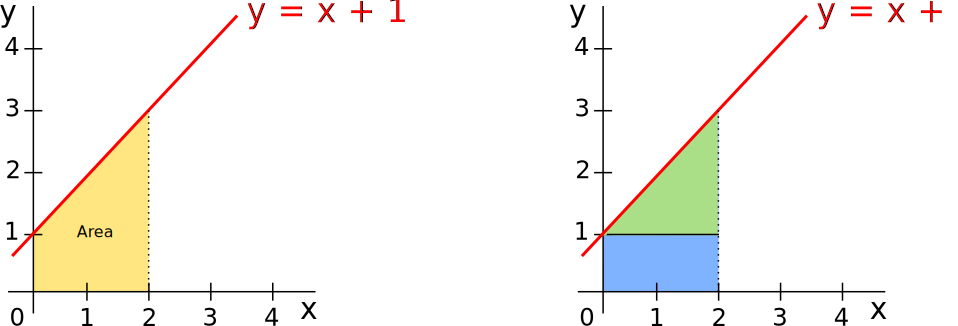
\includegraphics[width=5in]{images/int-ex}$$
Thus, the area is the sum of the areas of a rectangle and a triangle.
Hence,
\begin{eqnarray*}
\int_0^2 x+1~dx&=&\mbox{Net Area}\\
&=&\mbox{Area of rectangle} + \mbox{Area of triangle}\\
&=&(2)(1)+\frac{1}{2}(2)(2)\\
&=&4.
\end{eqnarray*}
\end{solution}



\subsection{The net change theorem} \index{net change theorem}

As we use the Fundamental Theorem of Calculus to evaluate definite integrals, it is essential that we remember and understand the meaning of the numbers we find.  We briefly summarize three key interpretations to date.
\begin{itemize}
	\item For a moving object with instantaneous velocity $v(t)$, the object's change in position on the time interval $[a,b]$ is given by $\int_a^b v(t) \, dt$, and whenever $v(t) \ge 0$ on $[a,b]$, $\int_a^b v(t) \, dt$ tells us the total distance traveled by the object on $[a,b]$.  
	\item For any continuous function $f$, its definite integral $\int_a^b f(x) \, dx$ represents the total net signed area bounded by $y = f(x)$ and the $x$-axis on $[a,b]$, where regions that lie below the $x$-axis have a minus sign associated with their area.  
%	\item The value of a definite integral is linked to the average value of a function: for a continuous function $f$ on $[a,b]$, its average value $f_{\mbox{\tiny{AVG}}[a,b]}$ is given by
%$$f_{\mbox{\tiny{AVG}}[a,b]} = \frac{1}{b-a} \int_a^b f(x) \, dx.$$
\end{itemize}
The Fundamental Theorem of Calculus now enables us to evaluate exactly (without taking a limit of Riemann sums) any definite integral for which we are able to find an antiderivative of the integrand.  

A slight change in notational perspective allows us to gain even more insight into the meaning of the definite integral.  To begin, recall Equation~(\ref{E:FTCV}), where we wrote the Fundamental Theorem of Calculus for a velocity function $v$ with antiderivative $V$ as
$$V(b) - V(a) = \int_a^b v(t) \, dt.$$
If we instead replace $V$ with $s$ (which represents position) and replace $v$ with $s'$ (since velocity is the derivative of position), Equation~(\ref{E:FTCV}) equivalently reads 
\begin{equation} \label{E:FTCs}
s(b) - s(a) = \int_a^b s'(t) \, dt.
\end{equation}
In words, this version of the FTC tells us that the net change in the object's position function on a particular interval is given by the definite integral of the position function's derivative over that interval.

Of course, this result is not limited to only the setting of position and velocity.  Writing the result in terms of a more general function $f$, we have the Net Change Theorem.

 \begin{theorem}{Net Change Theorem}{net_change_theorem} \index{net change theorem} If $f$ is a continuously differentiable function on $[a,b]$ with derivative $f'$, then 
 \begin{equation} \label{E:TotalChange}
f(b) - f(a) = \int_a^b f'(x) \, dx.
\end{equation}
That is, the  integral of the rate of change (derivative) of a function on $[a,b]$ is the net change of the function itself on $[a,b]$.
\end{theorem}

The Net Change Theorem tells us more about the relationship between the graph of a function and that of its derivative.  Recall from Chapter 4 that heights (or values) on the graph of the derivative function correspond to slopes on the graph of the function itself.  That observation occurred in the context where we knew $f$ and were seeking $f'$; if now instead we think about knowing $f'$ and seeking information about $f$, we can instead say the following:  
\begin{quote}
\emph{differences in heights on $f$ correspond to net signed areas bounded by $f'$.}
\end{quote}
\begin{figure}[h]
\begin{center}
\includegraphics{figures/4_4_TCT}
\caption{The graphs of $f'(x) = 4 - 2x$ (at left) and an antiderivative $f(x) = 4x - x^2$ at right.  Differences in heights on $f$ correspond to net signed areas bounded by $f'$.} \label{F:4.4.TCT}
\end{center}
\end{figure}
To see why this is so, say we consider the difference $f(1) - f(0)$.  Note that this value is $ 3 $, in part because $f(1) = 3$ and $f(0) = 0$, but also because the net signed area bounded by $y = f'(x)$ on $[0,1]$ is 3.  That is, $f(1) - f(0) = \int_0^1 f'(x) \, dx$.  A similar pattern holds throughout, including the fact that since the total net signed area bounded by $f'$ on $[0,4]$ is $0$, $\int_0^4 f'(x) \, dx = 0$, so it must be that $f(4) - f(0) = 0$, so $f(4) = f(0)$.

Beyond this general observation about area, the Net Change Theorem enables us to consider interesting and important problems where we know the rate of change, and answer key questions about the function whose rate of change we know. 

\begin{example} \label{Ex:4.4.1}
Suppose that pollutants are leaking out of an underground storage tank at a rate of $r(t)$ gallons/day, where $t$ is measured in days.  It is conjectured that $r(t)$ is given by the formula $r(t) = 0.0069t^3 -0.125t^2+11.079$ over a certain 12-day period.  The graph of $y=r(t)$ is given in Figure~\ref{F:4.4.TCTEx}.  What is the meaning of $\int_4^{10} r(t) \, dt$ and what is its value?  
%What is the average rate at which pollutants are leaving the tank on the time interval $4 \le t \le 10$?
\begin{figure}[h]
\begin{center}
\includegraphics{figures/4_4_TCTEx}
\caption{The rate $r(t)$ of pollution leaking from a tank, measured in gallons per day.} \label{F:4.4.TCTEx}
\end{center}
\end{figure}
\end{example}
\begin{solution}
We know that since $r(t) \ge 0$, the value of $\int_4^{10} r(t) \, dt$ is the area under the curve on the interval $[4,10]$.  If we think about this area from the perspective of a Riemann sum, the rectangles will have heights measured in gallons per day and widths measured in days, thus the area of each rectangle will have units of
$$\frac{\mbox{gallons}}{\mbox{day}} \cdot \mbox{days} = \mbox{gallons}.$$
Thus, the definite integral tells us the total number of gallons of pollutant that leak from the tank from day 4 to day 10.  The Net Change Theorem tells us the same thing:  if we let $R(t)$ denote the function that measures the total number of gallons of pollutant that have leaked from the tank up to day $t$, then $R'(t) = r(t)$, and 
$$\int_4^{10} r(t) \, dt = R(10) - R(4),$$
which is the net change in the function that measures total gallons leaked over time, thus the number of gallons that have leaked from day 4 to day 10.

To compute the exact value, we use the Fundamental Theorem of Calculus.  Antidifferentiating $r(t) = 0.0069t^3 -0.125t^2+11.079$, we find that
\begin{eqnarray*}
	\int_4^{10} (0.0069t^3 -0.125t^2+11.079) \, dt & = & \left. \left( 0.0069 \cdot \frac{1}{4} \, t^4 - 0.125 \cdot \frac{1}{3} t^3 + 11.079t \right) \right|_4^{10} \\
			& = & \left( 0.0069 \cdot \frac{1}{4} \, (10)^4 - 0.125 \cdot \frac{1}{3} (10)^3 + 11.079(10) \right) - \\
			& \ &  \left( 0.0069 \cdot \frac{1}{4} \, (4)^4 - 0.125 \cdot \frac{1}{3} (4)^3 + 11.079(4) \right) \\
			& \approx & 44.282. 
\end{eqnarray*}
Thus, approximately 44.282 gallons of pollutant leaked over the six day time period.

%To find the average rate at which pollutant leaked from the tank over $4 \le t \le 10$, we want to compute the average value of $r$ on $[4,10]$.  Thus,
%$$r_{\mbox{\tiny{AVG}}[4,10]} = \frac{1}{10-4} \int_4^{10} r(t) \, dt \approx \frac{44.282}{6} = 7.380,$$
%which has its units measured in gallons per day.
\end{solution}






Summary

\begin{itemize}
\item We can find the exact value of a definite integral without taking the limit of a Riemann sum or using a familiar area formula by finding the antiderivative of the integrand, and hence applying the Fundamental Theorem of Calculus.
\item The Fundamental Theorem of Calculus says that if $f$ is a continuous function on $[a,b]$ and $F$ is an antiderivative of $f$, then
$$\int_a^b f(x) \, dx = F(b) - F(a).$$
Hence, if we can find an antiderivative for the integrand $f$, evaluating the definite integral comes from simply computing the change in $F$ on $[a,b]$. 
\item A slightly different perspective on the FTC allows us to restate it as the Net Change Theorem, which says that
$$\int_a^b f'(x) \, dx = f(b) - f(a),$$
for any continuously differentiable function $f$.   This means that the definite integral of the instantaneous rate of change of a function $f$ on an interval $[a,b]$ is equal to the net change in the function $f$ on $[a,b]$.
\end{itemize}


\subsection{Functions defined by integrals}

The FTC enables us to compute the value of the antiderivative $F$ at a point $b$, provided that we know $F(a)$ and can evaluate the definite integral from $a$ to $b$ of $f$:
$$F(b) = F(a) + \int_a^b f(x) \, dx.$$
We may think of $b$, the upper limit of integration, as a variable itself.  To that end, we introduce the idea of an \emph{integral function}\index{integral function}, a function whose formula involves a definite integral.

Given a continuous function $f$, we define the corresponding integral function $A$ according to the rule 
\begin{equation} \label{E:intfxn}
A(x) = \int_a^x f(t) \, dt.
\end{equation}
Note particularly that because we are using the variable $x$ as the independent variable in the function $A$, and $x$ determines the other endpoint of the interval over which we integrate (starting from $a$), we need to use a variable other than $x$ as the variable of integration.  A standard choice is $t$, but any variable other than $x$ is acceptable.

One way to think of the function $A$ is as the ``net-signed area from $a$ up to $x$'' function, where we consider the region bounded by $y = f(t)$ on the relevant interval.  For example, in Figure~\ref{F:5.1.IntFxn}, we see a given function $f$ pictured at left, and its corresponding area function (choosing $a = 0$), $A(x) = \int_0^x f(t) \, dt$ shown at right.

\begin{figure}[h]
\begin{center}
\includegraphics{figures/5_1_IntFxn}
\end{center}
\caption{At left, the graph of the given function $f$.  At right, the area function $A(x) = \int_0^x f(t) \, dt$.} \label{F:5.1.IntFxn}
\end{figure}

Note particularly that the function $A$ measures the net-signed area from $t = 0$ to $t = x$ bounded by the curve $y = f(t)$; this value is then reported as the corresponding height on the graph of $y = A(x)$.  It is even more natural to think of this relationship between $f$ and $A$ dynamically.  At \href{http://gvsu.edu/s/cz}{\texttt{http://gvsu.edu/s/cz}}, we find a java applet\footnote{David Austin, Grand Valley State University} that brings the static picture in Figure~\ref{F:5.1.IntFxn} to life.  There, the user can move the red point on the function $f$ and see how the corresponding height changes at the light blue point on the graph of $A$.

% % % % % % % % % % % % % % % % % % % % % % % % % % % % %

\subsection{FTC 2} \label{sec:FTC2}

In the previous section we learned the Fundamental Theorem of Calculus (FTC), which from here forward will be referred to as the \emph{First} Fundamental Theorem of Calculus\index{Fundamental Theorem of Calculus!First}, as in this section we develop a corresponding result that follows it.

We begin by way of example. If we let $f(t) = \cos(t) - t$ and set $A(x) = \int_2^x f(t) \, dt$, then we can determine a formula for $A$ without integrals by the First FTC.  Specifically,
\begin{eqnarray*}
A(x) & = & \int_2^x (\cos(t) - t) \, dt \\
	& = & \sin(t) - \frac{1}{2}t^2 \bigg\vert_2^x \\
	& = & \sin(x) -  \frac{1}{2}x^2 - \left(\sin(2) - 2 \right).
\end{eqnarray*}
Differentiating $A(x)$, since $(\sin(2) - 2)$ is constant, it follows that 
$$A'(x) = \cos(x) - x,$$
and thus we see that $A'(x) = f(x)$.  This tells us that for this particular choice of $f$, $A$ is an antiderivative of $f$.  More specifically, since $A(2) = \int_2^2 f(t) \, dt = 0$, $A$ is the only antiderivative of $f$ for which $A(2) = 0$.

In general, if $f$ is any continuous function, and we define the function $A$ by the rule 
$$A(x) = \int_c^x f(t) \, dt,$$
where $c$ is an arbitrary constant, then we can show that $A$ is an antiderivative of $f$.  To see why, let's demonstrate that $A'(x) = f(x)$ by using the limit definition of the derivative.  Doing so, we observe that
\begin{align}
A'(x) &= \lim_{h \to 0} \frac{A(x+h) - A(x)}{h} \notag \\
	&= \lim_{h \to 0} \frac{\int_c^{x+h} f(t) \, dt - \int_c^x f(t) \, dt}{h} \notag \\
	&= \lim_{h \to 0} \frac{\int_x^{x+h} f(t) \, dt}{h}, \label{E:FTC2limdef}
\end{align}
where Equation~(\ref{E:FTC2limdef}) in the preceding chain follows from the fact that $\int_c^x f(t) \,dt + \int_x^{x+h} f(t) \, dt = \int_c^{x+h} f(t) \, dt$.  Now, observe that for small values of $h$,
$$\int_x^{x+h} f(t) \, dt \approx f(x) \cdot h,$$
by a simple left-hand approximation of the integral.  Thus, as we take the limit in Equation~(\ref{E:FTC2limdef}), it follows that
$$A'(x) =  \lim_{h \to 0} \frac{\int_x^{x+h} f(t) \, dt}{h} = \lim_{h \to 0} \frac{f(x) \cdot h}{h} = f(x).$$

%it follows from the First FTC that
%$$A(x) = F(x) - F(c).$$
%Since $F(c)$ is constant and $F$ is an antiderivative of $f$, we see
%$$A'(x) = F'(x) = f(x),$$
%and thus $A$ is an antiderivative of $f$.  

Hence, $A$ is indeed an antiderivative of $f$.  In addition, $A(c) = \int_c^c f(t) \, dt = 0.$  The preceding argument demonstrates the truth of the Second Fundamental Theorem of Calculus, which we state as follows.


\begin{theorem}{FTC 2}{fundamental_theorem_II} 
If $f$ is a continuous function and $a$ is any constant, then $f$ has a unique antiderivative $A$ that satisfies $A(a) = 0$, and that antiderivative is given by the rule $A(x) = \int_a^x f(t) \, dt$. That is to say
\[
A'(x) = \frac{d}{dx}\left[\int_c^x f(t) \, dt\right]= f(x) \text{ and } A(c)=0.
\]
\end{theorem}

We can prove the first version of the FTC using the second:

\begin{proof} Proof of Theorem~\ref{thm:fundamental_theorem_I}.

We know from Theorem~\ref{thm:fundamental_theorem_II} that 
$$
  A(x)=\int_a^x f(t)\,dt
$$
is an antiderivative of $f(x)$, and therefore any antiderivative
$F(x)$ of $f(x)$ is of the form $F(x)=A(x)+k$. Then 
\begin{eqnarray*}
  F(b)-F(a)=A(b)+k-(A(a)+k) &=& A(b)-A(a)\cr
  &=&\int_a^b f(t)\,dt-\int_a^a f(t)\,dt.\cr
\end{eqnarray*}
It is not hard to see that $\ds \int_a^a f(t)\,dt=0$, so this means that
$$
  F(b)-F(a)=\int_a^b f(t)\,dt,
$$
which is exactly what Theorem~\ref{thm:fundamental_theorem_I} says.
\end{proof}

\begin{example}{Using FTC}{UsingFTC}
\exfont{Differentiate} the following function:
$$g(x)=\int_{-2}^x \cos(1+5t)\sin t\,dt.$$
\end{example}

\begin{solution} 
We simply apply the Fundamental Theorem of Calculus directly to get:
$$g'(x)=\cos(1+5x)\sin x.$$
\end{solution}

Using the Chain Rule we can derive a formula for some more complicated problems.
If $ F$ is an antiderivative of $ f $, then we have:
$$\frac{d}{dx}\int_a^{v(x)}f(t)\,dt=\frac{d}{dx}\left(F(v(x))-F(a)\right) =f(v(x))\cdot v'(x) - 0=f(v(x))\cdot v'(x).$$

Now what if the upper limit is constant and the lower limit is a function of $x$?
Then we interchange the limits and add a minus sign to get:
$$\frac{d}{dx}\int_{u(x)}^af(t)\,dt=-\frac{d}{dx}\int_a^{u(x)} f(t)\,dt=-f(u(x))\cdot u'(x).$$

Combining these two we can get a formula where both limits are a function of $x$.
We break up the integral as follows:
$$\int_{u(x)}^{v(x)} f(t)\,dt=\int_{u(x)}^a f(t)\,dt+\int_a^{v(x)}f(t)\,dt.$$
We just need to make sure $f(a)$ exists after we break up the integral.
Then differentiating and using the above two formulas gives:

\begin{formulabox}[FTC I + Chain Rule:]
$$\frac{d}{dx}\int_{{u(x)}}^{{v(x)}} f(t)\,dt=f({v(x)}){v'(x)}-f({u(x)}){u'(x)}$$
\end{formulabox}

Many textbooks do not show this formula and instead to solve these types of problems will use FTC I along with the tricks we used to derive the formula above.
Either method is perfectly fine.

\begin{example}{FTC I + Chain Rule}{FTCIChainRule}
Differentiate the following integral:
$$\int_{10x}^{x^2} t^3\sin(1+t) \,dt.$$
\end{example}

\begin{solution} 
We will use the formula above.
We have $f(t)=t^3\sin(1+t)$, $u(x)=10x$ and $v(x)=x^2$.
Then $u'(x)=10$ and $v'(x)=2x$.
Thus,
\begin{eqnarray*}
\frac{d}{dx}\int_{10x}^{x^2} t^3\sin(1+t) \,dt&=&(x^2)^3\sin(1+(x^2))(2x)-(10x)^3\sin(1+(10x))(10)\\
\\
&=&2x^7\sin(1+x^2)-10000x^3\sin(1+10x)
\end{eqnarray*}
\end{solution}

\begin{example}{FTC I + Chain Rule}{FTCIChainRule2}
Differentiate the following integral with respect to $x$:
$$\int_{x^3}^{2x} 1+\cos t\,dt$$
\end{example}

\begin{solution} 
Using the formula we have:
$$\frac{d}{dx}\int_{x^3}^{2x} 1+\cos t\,dt=(1+\cos(2x))(2)-(1+\cos(x^3))(3x^2).$$
\end{solution}


\subsection{More on Differentiating Integral Functions}

The Second FTC provides us with a means to construct an antiderivative of any continuous function.  In particular, if we are given a continuous function $g$ and wish to find an antiderivative of $g$, we can now say that 
$$G(x) = \int_a^x g(t) \, dt$$
provides the rule for such an antiderivative, and moreover that $G(a) = 0$.  Note especially that we know that $G'(x) = g(x)$.  We sometimes want to write this relationship between $G$ and $g$ from a different notational perspective.  In particular, observe that
\begin{equation} \label{E:diffint}
\frac{d}{dx} \left[ \int_a^x g(t) \, dt \right] = g(x).
\end{equation}
This result can be particularly useful when we're given an integral function such as $G$ and wish to understand properties of its graph by recognizing that $G'(x) = g(x)$, while not necessarily being able to exactly evaluate the definite integral $\int_c^x g(t) \, dt$.

This shows that integral functions, while perhaps having the most complicated formulas of any functions we have encountered, are nonetheless particularly simple to differentiate.  For instance, if 
$$F(x) = \int_{\pi}^x \sin(t^2) \, dt,$$
then by the Second FTC, we know immediately that
$$F'(x) = \sin(x^2).$$

Stating this result more generally for an arbitrary function $f$, we know by the Second FTC that
$$\frac{d}{dx} \left[ \int_a^x f(t) \, dt \right] = f(x).$$
In words, the last equation essentially says that ``the derivative of the integral function whose integrand is $f$, is $f$.''  In this sense, we see that if we first integrate the function $f$ from $t = a$ to $t = x$, and then differentiate with respect to $x$, these two processes ``undo'' one another.

Taking a different approach, say we begin with a function $f(t)$ and differentiate with respect to $t$.  What happens if we follow this by integrating the result from $t = a$ to $t = x$?  That is, what can we say about the quantity
$$\int_a^x \frac{d}{dt} \left[ f(t) \right] \, dt?$$
Here, we use the First FTC and note that $f(t)$ is an antiderivative of $\frac{d}{dt} \left[ f(t) \right].$  Applying this result and evaluating the antiderivative function, we see that
\begin{eqnarray*}
\int_a^x \frac{d}{dt} \left[ f(t) \right] \, dt & = & f(t) \bigg\vert_a^x \\
							& = & f(x) - f(a).
\end{eqnarray*} 
Thus, we see that if we apply the processes of first differentiating $f$ and then integrating the result from $a$ to $x$, we return to the function $f$, minus the constant value $f(a)$.  So in this situation, the two processes almost undo one another, up to the constant $f(a)$.

The observations made in the preceding two paragraphs demonstrate that differentiating and integrating (where we integrate from a constant up to a variable) are almost inverse processes.  In one sense, this should not be surprising:  integrating involves antidifferentiating, which reverses the process of differentiating.  On the other hand, we see that there is some subtlety involved, as integrating the derivative of a function does not quite produce the function itself.  This is connected to a key fact  that any function has an infinite family of antiderivatives, and any two of those antiderivatives differ only by a constant.


% % % % % % % % % % % % % % % % % % % % % % % % % % % % % %

%Let's rewrite this slightly: 
%$$
%  \int_a^x f(t)\,dt = F(x)-F(a).
%$$
%We've replaced the variable $x$ by $t$ and $b$ by $x$. These are just
%different names for quantities, so the substitution doesn't change the
%meaning. It does make it easier to think of the two sides of the
%equation as functions. The expression
%$$
%  \int_a^x f(t)\,dt
%$$
%is a function: plug in a value for $x$, get out some other value. The
%expression $F(x)-F(a)$ is of course also a function, and it has a nice
%property: 
%$$
%  {d\over dx} (F(x)-F(a)) = F'(x) = f(x),
%$$
%since $F(a)$ is a constant and has derivative zero. In other words, by
%shifting our point of view slightly, we see that the odd looking
%function
%$$
%  G(x)=\int_a^x f(t)\,dt
%$$
%has a derivative, and that in fact $G'(x)=f(x)$. This is really just a
%restatement of the Fundamental Theorem of Calculus, and indeed is
%often called the Fundamental Theorem of Calculus. To avoid confusion,
%some people call the two versions of the theorem ``The Fundamental
%Theorem of Calculus, part I'' and ``The Fundamental
%Theorem of Calculus, part II'', although unfortunately there is no
%universal agreement as to which is part I and which part II. Since it
%really is the same theorem, differently stated, some people simply
%call them both ``The Fundamental
%Theorem of Calculus.''
%
%\begin{theorem}{Fundamental Theorem of Calculus}{fundamental_theorem_II}
%Suppose that $f(x)$ is
%continuous on the interval $[a,b]$ and let
%$$
%  G(x)=\int_a^x f(t)\,dt.
%$$
%Then $G'(x)=f(x)$.
%\end{theorem}
%
%We have not really proved the Fundamental Theorem. In a nutshell, we
%gave the following argument to justify it: Suppose we want to know the
%value of 
%$$
%  \int_a^b f(t)\,dt = \lim_{n\to\infty}\sum_{i=0}^{n-1} f(t_i)\Delta t.
%$$
%We can interpret the right hand side as the distance traveled by an
%object whose speed is given by $f(t)$. We know another way to compute
%the answer to such a problem: find the position of the object by
%finding an antiderivative of $f(t)$, then substitute $t=a$ and $t=b$
%and subtract to find the distance traveled. This must be the answer to
%the original problem as well, even if $f(t)$ does not represent a
%speed.
%
%What's wrong with this? In some sense, nothing. As a practical matter
%it is a very convincing argument, because our understanding of the
%relationship between speed and distance seems to be quite solid. From
%the point of view of mathematics, however, it is unsatisfactory to
%justify a purely mathematical relationship by appealing to our
%understanding of the physical universe, which could, however unlikely
%it is in this case, be wrong.
%
%A complete proof is a bit too involved to include here, but we will
%indicate how it goes. First, if we can prove the second version of the
%Fundamental Theorem, Theorem~\ref{thm:fundamental_theorem_II}, then
%we can prove the first version from that:
%
%\begin{proof} Proof of Theorem~\ref{thm:fundamental_theorem_I}.
%
%We know from Theorem~\ref{thm:fundamental_theorem_II} that 
%$$
%  G(x)=\int_a^x f(t)\,dt
%$$
%is an antiderivative of $f(x)$, and therefore any antiderivative
%$F(x)$ of $f(x)$ is of the form $F(x)=G(x)+k$. Then 
%\begin{eqnarray*}
%  F(b)-F(a)=G(b)+k-(G(a)+k) &=& G(b)-G(a)\cr
%  &=&\int_a^b f(t)\,dt-\int_a^a f(t)\,dt.\cr
%\end{eqnarray*}
%It is not hard to see that $\ds \int_a^a f(t)\,dt=0$, so this means that
%$$
%  F(b)-F(a)=\int_a^b f(t)\,dt,
%$$
%which is exactly what Theorem~\ref{thm:fundamental_theorem_I} says.
%\end{proof}
%
%So the real job is to prove
%Theorem~\ref{thm:fundamental_theorem_II}. We will sketch the proof,
%using some facts that we do not prove. First, the following identity
%is true of integrals:
%$$
%  \int_a^b f(t)\,dt = \int_a^c f(t)\,dt + \int_c^b f(t)\,dt.
%$$
%This can be proved directly from the definition of the integral, that
%is, using the limits of sums. It is quite easy to see that it must be
%true by thinking of either of the two applications of integrals that
%we have seen. It turns out that the identity is true no matter what
%$c$ is, but it is easiest to think about the meaning when 
%$a\le c\le b$.
%
%First, if $f(t)$ represents a speed, then we know that the three
%integrals represent the distance traveled between time $a$ and time $b$;
%the distance traveled between time $a$ and time $c$; and 
%the distance traveled between time $c$ and time $b$. Clearly the sum of
%the latter two is equal to the first of these.
%
%Second, if $f(t)$ represents the height of a curve, the three
%integrals represent the area under the curve between $a$ and $b$;
%the area under the curve between $a$ and $c$;
%and the area under the curve between $c$ and $b$. Again it is clear
%from the geometry that the first is equal to the sum of the second and
%third. 
%
%\begin{proof} Proof of Theorem~\ref{thm:fundamental_theorem_II}.
%
%We want to compute $G'(x)$, so we start with the definition of the
%derivative in terms of a limit:
%\begin{eqnarray*}
%  G'(x)&=&\lim_{\Delta x\to0}{G(x+\Delta x)-G(x)\over\Delta x}\cr
%  &=&\lim_{\Delta x\to0}{1\over \Delta x}\left(
%  \int_a^{x+\Delta x} f(t)\,dt - \int_a^x f(t)\,dt\right)\cr
%  &=&\lim_{\Delta x\to0}{1\over \Delta x}\left(
%  \int_a^{x} f(t)\,dt + \int_x^{x+\Delta x} f(t)\,dt - 
%  \int_a^x f(t)\,dt\right)\cr
%  &=&\lim_{\Delta x\to0}{1\over \Delta x}\int_x^{x+\Delta x} f(t)\,dt.\cr
%\end{eqnarray*}
%Now we need to know something about 
%$$
%  \int_x^{x+\Delta x} f(t)\,dt
%$$
%when $\Delta x$ is small; in fact, it is very close to 
%$\Delta x f(x)$, but we will not prove this. Once again, it is easy to
%believe this is true by thinking of our two applications:
%The integral 
%$$
%  \int_x^{x+\Delta x} f(t)\,dt
%$$
%can be interpreted as the distance traveled by an object over a very
%short interval of time. Over a sufficiently short period of time, the
%speed of the object will not change very much, so the distance
%traveled will be approximately the length of time multiplied by the
%speed at the beginning of the interval, namely, $\Delta x
%f(x)$. Alternately, the integral may be interpreted as the area under
%the curve between $x$ and $x+\Delta x$. When $\Delta x$ is very small,
%this will be very close to the area of the rectangle with base $\Delta
%x$ and height $f(x)$; again this is $\Delta x
%f(x)$. If we accept this, we may proceed:
%$$
%  \lim_{\Delta x\to0}{1\over \Delta x}\int_x^{x+\Delta x} f(t)\,dt
%  =\lim_{\Delta x\to0}{\Delta x f(x)\over \Delta x}=f(x),
%$$
%which is what we wanted to show.
%\end{proof}
%
%It is still true that we are depending on an interpretation of the
%integral to justify the argument, but we have isolated this part of
%the argument into two facts that are not too hard to prove. Once the
%last reference to interpretation has been removed from the proofs of
%these facts, we will have a real proof of the Fundamental Theorem.
%
%Now we know that to solve certain kinds of problems, those that lead
%to a sum of a certain form, we ``merely'' find an antiderivative and
%substitute two values and subtract. Unfortunately, finding
%antiderivatives can be quite difficult. While there are a small number
%of rules that allow us to compute the derivative of any common
%function, there are no such rules for antiderivatives. There are some
%techniques that frequently prove useful, but we will never be able to
%reduce the problem to a completely mechanical process.
%
%Due to the close relationship between an integral and an
%antiderivative, the integral sign is also used to mean
%``antiderivative''. You can tell which is intended by whether the
%limits of integration are included:
%$$
%  \int_1^2 x^2\,dx
%$$
%is an ordinary integral, also called a 
%\dfont{definite integral},
%because it has a definite value, namely
%$$
%  \int_1^2 x^2\,dx={2^3\over3}-{1^3\over3}={7\over3}.
%$$
%We use
%$$
%  \int x^2\,dx
%$$
%to denote the antiderivative of $\ds x^2$, also called an
%\dfont{indefinite integral}.
%So this is evaluated as
%$$
%  \int x^2\,dx = {x^3\over 3}+C.
%$$
%It is customary to include the constant $C$ to indicate that there are
%really an infinite number of antiderivatives. We do not need this $C$
%to compute definite integrals, but in other circumstances we will need
%to remember that the $C$ is there, so it is best to get into the habit
%of writing the $C$.
%When we compute a definite integral, we first find an antiderivative
%and then substitute. It is convenient to first display the
%antiderivative and then do the substitution; we need a notation
%indicating that the substitution is yet to be done. A typical solution
%would look like this:
%$$
%  \int_1^2 x^2\,dx=\left.{x^3\over 3}\right|_1^2 = 
%  {2^3\over3}-{1^3\over3}={7\over3}.
%$$
%The vertical line with subscript and superscript is used to indicate
%the operation ``substitute and subtract'' that is needed to finish the
%evaluation.
%
%We seem to have found a pattern. When attempting to solve a previous question, we found the antiderivative of $x^2$ to be $x^3/3+c$ (as it was when solving the indefinite integral). Likewise, when we first began, we were trying to determine a position based on velocity, and $3t$ gave rise to $3t^2/2+k$.
%
%As will be formalized later, we see that in these cases, the power is increased to $n+1$, but we also divide through by this factor, $n+1$. So $x$ becomes $x^2/2$, $x^2$ becomes $x^3/3$, and $x^3$ will become $x^4/4$.
%
%Now we will also try with negative and fraction values in the following example.

%\begin{example}{Fundamental Theorem of Calculus}{FundamentalTheoremCalculus}
%Evaluate $\ds\int_1^4 x^3+\sqrt{x}+\frac{1}{x^2}\,dx $.
%\end{example}
%
%\begin{solution}
%\[ \begin{array}{lcl}
%\ds\int_1^4 x^3+\sqrt{x}+\frac{1}{x^2}\,dx 
%	& = & \ds\left.\frac{x^4}{4}+\frac{2x^{3/2}}{3}-x^{-1}\right|_1^4\\
%\\
%	& = & \ds\left(\frac{(4)^4}{4}+\frac{2(4)^{3/2}}{3}-4^{-1}\right) \\
%\\
%	& & \ds-\left(\frac{(1)^4}{4}+\frac{2(1)^{3/2}}{3}-1^{-1}\right)\\
%\\
%	& = & \ds\frac{415}{6}
%\end{array}\]\
%\end{solution}

%\begin{formulabox}[Properties of Definite Integrals]
%Some properties are as follows:
%$$\mbox{Order of limits matters:}\qquad\int_a^b f(x)\,dx=-\int_b^a f(x)\,dx$$
%$$\mbox{If interval is empty, integral is zero:}\qquad\int_a^a f(x)\,dx=0$$
%$$\mbox{Constant Multiple Rule:}\qquad\int_a^b cf(x)\,dx=c\int_a^b f(x)\,dx$$
%$$\mbox{Sum/Difference Rule:}\qquad\int_a^b f(x)\pm g(x)\,dx=\int_a^b f(x)\,dx\pm\int_a^b g(x)\,dx$$
%$$\mbox{Can split up interval $[a,b]=[a,c]\cup[c,b]$:}\qquad\int_a^b f(x)\,dx=\int_a^c f(x)\,dx+\int_c^b f(x)\,dx$$
%$$\mbox{The variable does not matter!:}\qquad\int_a^b f(x)\,dx=\int_a^b f(t)\,dt$$
%\end{formulabox}
%
%The reason for the last property is that a definite integral is a \ifont{number}, not a function, so the variable is just a placeholder that won't appear in the final answer.
%
%Some additional properties are \ifont{comparison} types of properties.
%
%\begin{formulabox}[Comparison Properties of Definite Integrals]
%$$\mbox{If $f(x)\geq 0$ for $x\in[a,b]$, then:}\qquad\int_a^b f(x)\,dx\geq 0.$$
%$$\mbox{If $f(x)\geq g(x)$ for $x\in[a,b]$, then:}\qquad\int_a^b f(x)\,dx\geq \int_a^b g(x)\,dx.$$
%$$\mbox{If $m\leq f(x)\leq M$ for $x\in[a,b]$, then:}\qquad m(b-a)\leq \int_a^b f(x)\,dx\leq M(b-a).$$
%\end{formulabox}
%
%\begin{example}{Properties of Definite Integrals}{PropertiesDefiniteIntegrals}
%Suppose $\ds{\int_a^b f(x)~dx=7}$ and $\ds{\int_a^b g(x)~dx=3}$. Find:
%\begin{multicols}{2}
%\begin{enumerate}
%	\item	$\ds\int_a^b 2f(x)-3g(x)\,dx$.
%	\item	$\ds\int_{b}^{a} 2g(x)\,dx$.
%	\item	$\ds\int_a^a f(x)\cdot g(x)\,dx$.
%	\item	$\ds\int_a^c f(x)~dx+\int_c^b f(x)\,dx$.
%\end{enumerate}
%\end{multicols}
%\vspace{5mm}
%\end{example}
%\begin{solution}
%\begin{enumerate}
%	\item	$\ds\int_a^b 2f(x)-3g(x)\,dx=\ds 2\int_a^b f(x)\,dx-3\int_a^b g(x)\,dx=2(7)-3(3)=5$.
%	\item	$\ds\int_{b}^{a} 2g(x)\,dx=\ds -2\int_{a}^{b} g(x)\,dx=-2(3)=-6$.
%	\item	$\ds\int_a^a f(x)\cdot g(x)\,dx=0$.
%	\item	$\ds\int_a^c f(x)\,dx+\int_c^b f(x)\,dx=\ds\int_a^b f(x)\,dx=7$.
%\end{enumerate}
%\end{solution}

%We next evaluate a definite integral using three different techniques.
%
%
%We next apply FTC to differentiate a function.


This section has laid the groundwork for a lot of great mathematics to follow. The most important lesson is this: definite integrals can be evaluated using antiderivatives. Since the previous section established that definite integrals are the limit of Riemann sums, we can later create Riemann sums to approximate values other than ``area under the curve,'' convert the sums to definite integrals, then evaluate these using the Fundamental Theorem of Calculus. This will allow us to compute the work done by a variable force, the volume of certain solids, the arc length of curves, and more.

The downside is this: generally speaking, computing antiderivatives is much more difficult than computing derivatives. The next chapter is devoted to techniques of finding antiderivatives so that a wide variety of definite integrals can be evaluated. Before that, the next section explores techniques of approximating the value of definite integrals beyond using the Left Hand, Right Hand and Midpoint Rules.

%%%%%%%%%%%%%%%%%%%%%%%%%%%%%%%%%%%%%%%%%%%%%%%%%
\Opensolutionfile{solutions}[ex]
\section*{Exercises for Section \ref{sec:FTC}}

\begin{enumialphparenastyle}

%%%%%%%%%%
\begin{ex}
Evaluate $\ds \int_1^4 t^2+3t\,dt$
\begin{sol}
 $87/2$
\end{sol}
\end{ex}

%%%%%%%%%%
\begin{ex}
Evaluate $\ds \int_0^\pi \sin t\,dt$
\begin{sol}
 $2$
\end{sol}
\end{ex}

%%%%%%%%%%
\begin{ex}
Evaluate $\ds \int_1^{10} {1\over x}\,dx$
\begin{sol}
 $\ln(10)$
\end{sol}
\end{ex}

%%%%%%%%%%
\begin{ex}
Evaluate $\ds \int_0^5 e^x\,dx$
\begin{sol}
 $\ds e^5-1$
\end{sol}
\end{ex}

%%%%%%%%%%
\begin{ex}
Evaluate $\ds \int_0^3 x^3\,dx$
\begin{sol}
 $\ds 3^4/4$
\end{sol}
\end{ex}

%%%%%%%%%%
\begin{ex}
Evaluate $\ds \int_1^2 x^5\,dx$
\begin{sol}
 $\ds 2^6/6 -1/6$
\end{sol}
\end{ex}

%%%%%%%%%%
\begin{ex}
 Find the derivative of $\ds G(x)=\int_1^x t^2-3t\,dt$
\begin{sol}
 $\ds x^2-3x$
\end{sol}
\end{ex}

%%%%%%%%%%
\begin{ex}
 Find the derivative of $\ds G(x)=\int_1^{x^2} t^2-3t\,dt$
\begin{sol}
 $\ds 2x(x^4-3x^2)$
\end{sol}
\end{ex}

%%%%%%%%%%
\begin{ex}
 Find the derivative of $\ds G(x)=\int_1^x e^{t^2}\,dt$
\begin{sol}
 $\ds e^{x^2}$
\end{sol}
\end{ex}

%%%%%%%%%%
\begin{ex}
 Find the derivative of $\ds G(x)=\int_1^{x^2} e^{t^2}\,dt$
\begin{sol}
 $\ds 2xe^{x^4}$
\end{sol}
\end{ex}

%%%%%%%%%%
\begin{ex}
 Find the derivative of $\ds G(x)=\int_1^x \tan(t^2)\,dt$
\begin{sol}
 $\ds \tan(x^2)$
\end{sol}
\end{ex}

%%%%%%%%%%
\begin{ex}
 Find the derivative of $\ds G(x)=\int_{10x}^{x^2} \tan(t^2)\,dt$
\begin{sol}
 $\ds 2x\tan(x^4)-10\tan(100x^2)$
\end{sol}
\end{ex}

%%%%%%%%%%
\begin{ex}
Suppose $\int_{1}^{4}f(x)\,dx=2$ and $\int_{1}^{4}g(x)\,dx=7$. Find $\int_{1}^{4}(5f(x)+3g(x))\,dx$ and $\int_{1}^{4}(6-2f(x))\,dx$.
\begin{sol}
	31, 14
\end{sol}
\end{ex}

%%%%%%%%%%
\begin{ex}
Suppose $\int_{-2}^{5}f(x)\,dx=3$ and $\int_{1}^{5}f(x)\,dx=-2$. Find $\int_{-2}^{1}f(x)\,dx$.
\begin{sol}
	5
\end{sol}
\end{ex}

%%%%%%%%%%
\begin{ex}
If $f$ is continuous on $[a,b]$, we define the average of $f(x)$ on $[a,b]$ to be
\begin{equation*}
\text{avg}_{[a,b]}(f)=\frac{1}{b-a}\int_{a}^{b}f(x)\,dx.
\end{equation*}
\begin{enumerate}
	\item	What is the average of $\sqrt{x}$ on the interval $[0,1]?$
	\item	If the average of $f(x)$ on $[0,2]$ and on $[2,5]$ are 6 and 4 respectively, then what is its average on $[0,5]$?
\end{enumerate}
\begin{sol}
\begin{enumerate}
	\item	2/3
	\item	24/5
\end{enumerate}
\end{sol}
\end{ex}

\end{enumialphparenastyle}